\documentclass[mim_thesis.tex]{subfiles} 
\begin{document}

The subsections on this chapter explain how to create an account on ADL Designer, the web-tool used for parsing the openEHR resources, and how to connect a repository with it. Are also explained the steps taken for the development of the script made for archetypes compliance and comparison from a local repository with the GitHub mirror of openEHR CKM.  

\section{Programming Technologies}
After analyzed all the materials that were provided, was decided that the best platform for the script would be by using an web browser, due to its practicality for an ordinary user. It was used the Angular 2 framework, together with the REST API calls that could be made to ADL Designer web tool/application, which works as a \textit{middleware} for fetching resources from the local repositories, and to GitHub openEHR CKM repository, along with all the materials mentioned on \textit{Materials and Methods} chapter. For this, was created a web-page that can run this script in the background, after using the credentials from ADL Designer for login and authentication.

\subsection{Script process and methodology}

Before running the script, it is necessary to create an account on ADL Designer and connect the local repository to it. If the repository of openEHR resources is not connected to this tool, the script it will not work, since it is dependent from it.

\subsubsection{Creating an account}
The official web-page for ADL Designer is \url{https://ehrscape.marand.si/designerv2}. It has a default account that can be logged in for testing purposes. To have a personal account is necessary to request it at \url{https://www.ehrscape.com/register.html}.
After getting an account, it is necessary to connect the desired repository to ADL Designer. It offers connection to various cloud repositories like OneDrive, Google Drive, Dropbox, GitHub, Bitbucket, Box and other CVS systems like GIT or connection to a local folder in a local machine. Depending on the chosen repository, other fields needs to be filled up as seen in figure \ref{fig:adl_designer_repositories}

\begin{figure}[H]
	\centering
    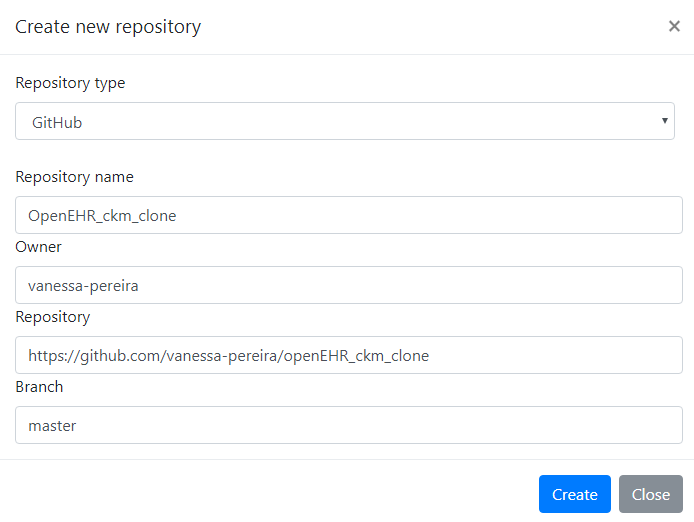
\includegraphics[width=0.9\textwidth]{img/adl_designer_repositories.PNG}
	\caption{Configuring repository connection on ADL Designer}
	\label{fig:adl_designer_repositories}
\end{figure}

With this, the openEHR based repository is created and connected to ADL Designer and ready to be also connected to the compliance comparison script. The repository name will be identified as \textit{"repositoryID"} parameter inside of the script code.

\subsubsection{Script Algorithm}
The algorithm of the script works as follows:
\begin{enumerate}[noitemsep]
\item Connect and authenticate to ADL Designer (\textit{user:password});
\item Connect to repository inside of ADL Designer (\textit{repositoryID});
\item GET method call to ADL Designer to get the list of archetypes and templates from the local repository;
\item Parse the object obtained from the previous call by \textit{archetypeID}, \textit{UID}, \textit{rmType}, \textit{MD5-CAM-1.0.1}, \textit{build\_uid}, \textit{revision};
\item GET method call for raw file URL from GitHub, that allows the archetype comparison;
\item Differentiate the URL paths for each archetype RM type;
\item Make comparison between versions on both repositories and return the new ones that can be found on GitHub;
\item Present results for archetype comparison (compliant or not compliant) and in case of-non internal archetype, return the GitHub URL for the new version of archetype in ADL RAW format.
\end{enumerate}
 
 The figure \ref{fig:script_process} shows the previous steps in a \ac{BPMN}:
 
\begin{figure}[H]
	\centering
    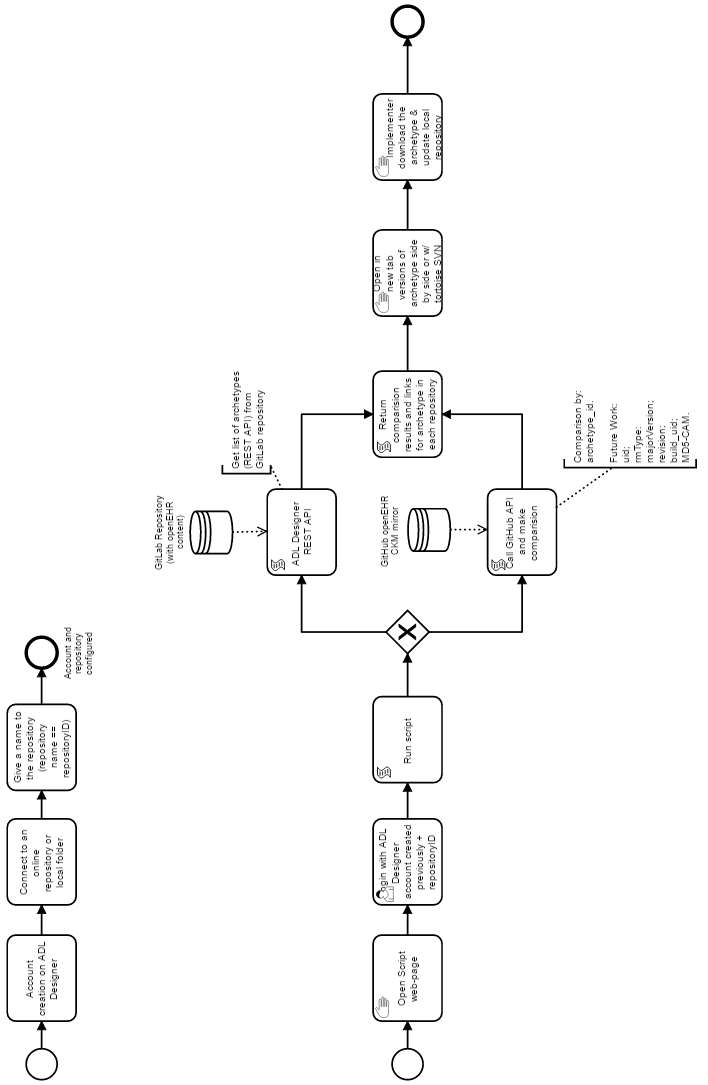
\includegraphics[width=1.07\textwidth]{img/script_process.PNG}
	\caption{Script Process}
	\label{fig:script_process}
\end{figure}

\section{Development}
The script developed was based on the information taken from the objects retrieved by the REST API GET calls of archetypes and templates from ADL Designer to the local repository, and from the structure study of openEHR CKM on GitHub, available on Chapter 3 - OpenEHR CKM. The information is analyzed by the script and it returns the URLs from the updated archetype versions available at openEHR CKM mirror account. At this stage, the script only analyze and presents the archetypes from the openEHR CKM instance of the openEHR Foundation (Publisher Namespace/Custodian Organization: org.openEHR) and only present at the "local" folder (see image \ref{fig:CKM_mirror_organization}).

The classes created to received the information from the calls are presented at table \ref{tab:adl_designer_calls}, together with an example of the data received by each parameter.

\begin{table}[H]
\caption{Classes "Archetypes" and "Templates" used to get information from ADL Designer calls}
\label{tab:adl_designer_calls}
\centering
\begin{tabular}{l}
\toprule[2pt]
\begin{lstlisting}[language=java]
  
  export class Archetypes {
  
    dataResponse: string;  		// full response from ADL Designer
    archetypeId: string; 	 	// e.g. openEHR-EHR-SECTION.adhoc.v1
    path: string; 			// e.g. openEHR-EHR-SECTION.adhoc.v1.adl
    rmType: string; 			// e.g. SECTION
    uid: string; 			// e.g. a82233b9-7f2d-4dd5-8db4-37f6963cfd8c
    details: ["MD5-CAM-1.0.1"]; build_uid; revision: string;
    dependsOn;
    specializedArch : string;
    urlGithubReturn;
    sumArchError;
    sumArchOK : number;
    temp_val;
    
  }


  export class Templates {
  
    dataResponse: string;  		// full response from ADL Designer
    templateId: string;  		// e.g. Vital Signs Measurement Request
    uid: string; 			// e.g. aa69c166-ebbd-48d2-bbfe-9fba97ddfbea
    dependsOn;
    archetypes;
    temp_val;
    
  }
  
\end{lstlisting}
\tabularnewline \bottomrule[2pt]
\end{tabular}
\end{table}

Owing to the repository chosen for testing and proof of concept be connected to a local database hosted at GitLab, the "archetypeID", "path" and "rmType" parameters allowed to construct and retrieve the URL link for each archetype for future comparison. Since it is a private repository, it will require credentials for authentication. 

For the searching component on the openEHR CKM mirror repository, the "rmType" parameter allowed to decide on which URL the archetype should be searched. In case on archetypes with the "rmType" paramater equal to "ACTION", "EVALUATION", "OBSERVATION", "INSTRUCTION" and "ADMIN\_ENTRY", the URL from GitHub should have appended the folder "Entry". In the other "rmType" cases, this was not necessary. The management of both cases can be seen in table \ref{tab:code_calls}. 

\begin{table}[H]
\caption{GET method calls, transformations and search}
\label{tab:code_calls}
\centering
\begin{tabular}{l}
\toprule[2pt]
\begin{lstlisting}[language=java]
//(...)

      this.http.get(githubBaseUrl + this.archetypeLists[i].rmType.toLowerCase() + '/' + 
      this.archetypeLists[i].archetypeId + '.adl', options)
        .subscribe(
        
        response1 => {
          archetypeLists[i].temp_val = response.text().startsWith('archetype') ? imgOk + 
          statusUpd : imgNotOk + statusOut;
        },

        response2 => {
          if (this.archetypeLists[i].rmType.toLowerCase() === 'action' || 'observation' || 
          'admin_entry' || 'evaluation' || 'instruction') {
            this.http.get(githubBaseUrl + 'entry/' + 
            this.archetypeLists[i].rmType.toLowerCase() + '/' + 
            this.archetypeLists[i].archetypeId + '.adl')
              .subscribe(
              response => {
                archetypeLists[i].temp_val = response.text().startsWith('archetype') ? imgOk + 
                statusUpd : imgNotOk + statusOut;
              },
              
//(...)

                  switch (this.archetypeLists[i].rmType.toLowerCase()) {
                    case "action":
                    case "observation":
                    case "admin_entry":
                    case "evaluation":
                    case "instruction":
                      url = githubBaseUrl + 'entry/' + 
                      this.archetypeLists[i].rmType.toLowerCase() + '/' + 
                      this.archetypeLists[i].archetypeId + '.adl';
                      break;
                    default:
                      url = githubBaseUrl +
                      this.archetypeLists[i].rmType.toLowerCase() + '/' + 
                      this.archetypeLists[i].archetypeId + '.adl';  
                      break;
                  }

                  if (url.indexOf(".v0") > 0) {
                    var urlGithub = url.replace("v0", "v1");
                    console.log(urlGithub);
                    return this.http.get(urlGithub)
                      .subscribe(
                      data => archetypeLists[i].urlGithubReturn = urlGithub,
                      error => { archetypeLists[i].urlGithubReturn = (error.status === 200) ? 
                      urlGithub : "Internal Archetype" }
                      
                      );
                  }
                  
                  if (url.indexOf(".v1") > 0) {
                    var urlGithub = url.replace("v1", "v0");
                    return this.http.get(urlGithub)
                      .subscribe(
                      data => archetypeLists[i].urlGithubReturn = urlGithub,
                      error => {
                        var urlGithub = url.replace("v1", "v2");
                        return this.http.get(urlGithub)
                          .subscribe(
                          data => { archetypeLists[i].urlGithubReturn = urlGithub },
                          error => { archetypeLists[i].urlGithubReturn = 
                          (error.status === 200) ? urlGithub : "Internal Archetype" }
//(...)
                        );
                      },
                    );
                  }
\end{lstlisting}
\tabularnewline \bottomrule[2pt]
\end{tabular}
\end{table}

With this, when the search by \textit{archetype\_id} is made to the openEHR CKM GitHub repository, the script will always return the URL of the latest version available, even in cases where the major version has been wrongly increased or decrease by some person responsible on the governance of the local repository. 


\section{Results}

The results can be seen live at \url{https://mim-script-openehr.stackblitz.io/}.

The login section is situated on the top of the page, where the script will run. A small introduction about the motivation of creating this script was made, along with the information of how to use it. In the next figures is possible to see how the page was designed together with the results retrieved from the script, after analyzing the local repository mentioned on the \textit{Material and Methods} chapter. 

\begin{figure}[H]
	\centering
    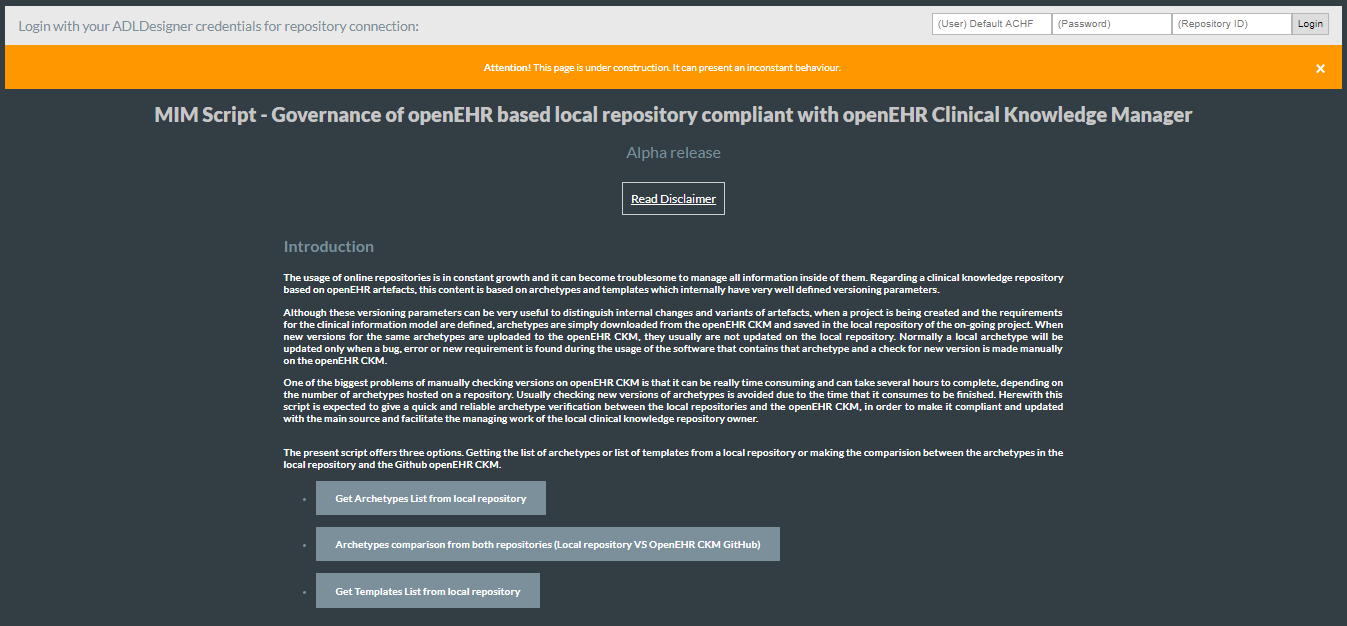
\includegraphics[width=1\textwidth]{img/script_main_page.PNG}
	\caption{Script Main Page }
	\label{fig:script_main_page}
\end{figure}

The script web-page was divided in 3 main sections: 

\begin{enumerate}[noitemsep]
\item Get Archetypes list from local repository;
\item Comparison from local repository and compliance with the openEHR CKM mirror at Github;
\item Get Templates list from local repository; 
\end{enumerate}

All these sections are dependent on the successful login made previously, otherwise the web page will present a never-ending loading logo under each section, until the login credentials are correctly inserted. \\

The first section contains a table with a list of archetypes from the local repository, with the respective \textit{UID}, \textit{MD5-CAM} hash, \textit{build\_uid} and \textit{revision} parameters, and the URL to the local repository for a quick user access. Also, each parameter presents a small explanation of its meaning. 

\begin{figure}[H]
	\centering
    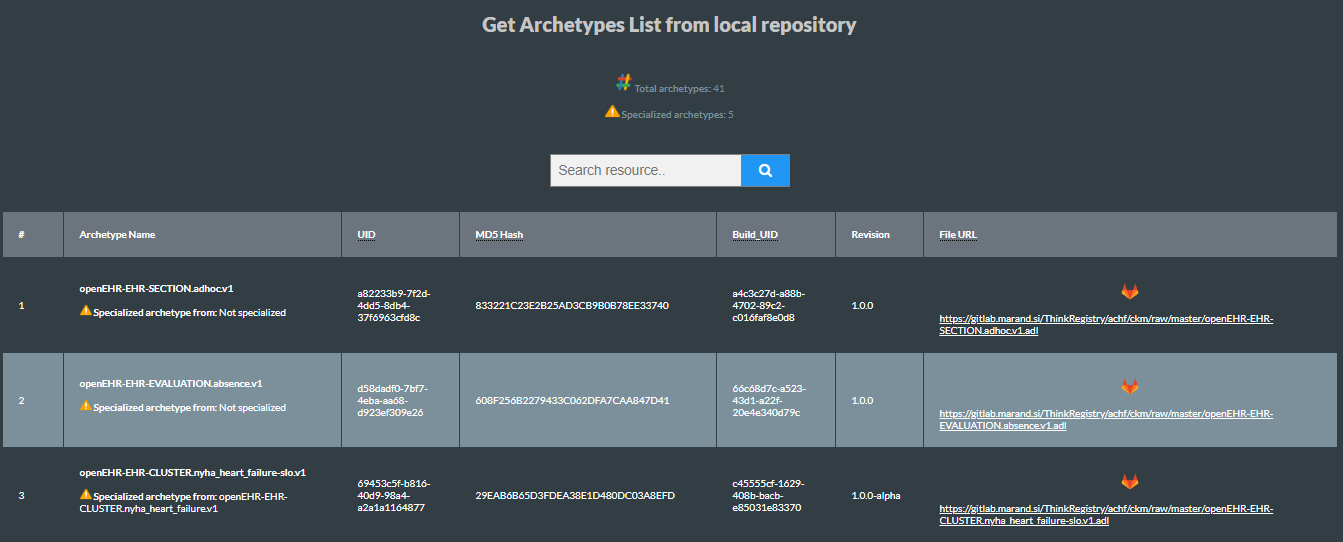
\includegraphics[width=1\textwidth]{img/get_arch_list.PNG}
	\caption{Module Get Archetypes list from local repository }
	\label{fig:get_arch_list}
\end{figure}

The second section presents the list of archetypes from the local repository (\textit{archetype\_id} and \textit{UID}) with the comparison result, that in case of outdated archetype, it returns the URL to the newest version on the GitHub openEHR CKM, along with the link to the version in the local repository. 

\begin{figure}[H]
	\centering
    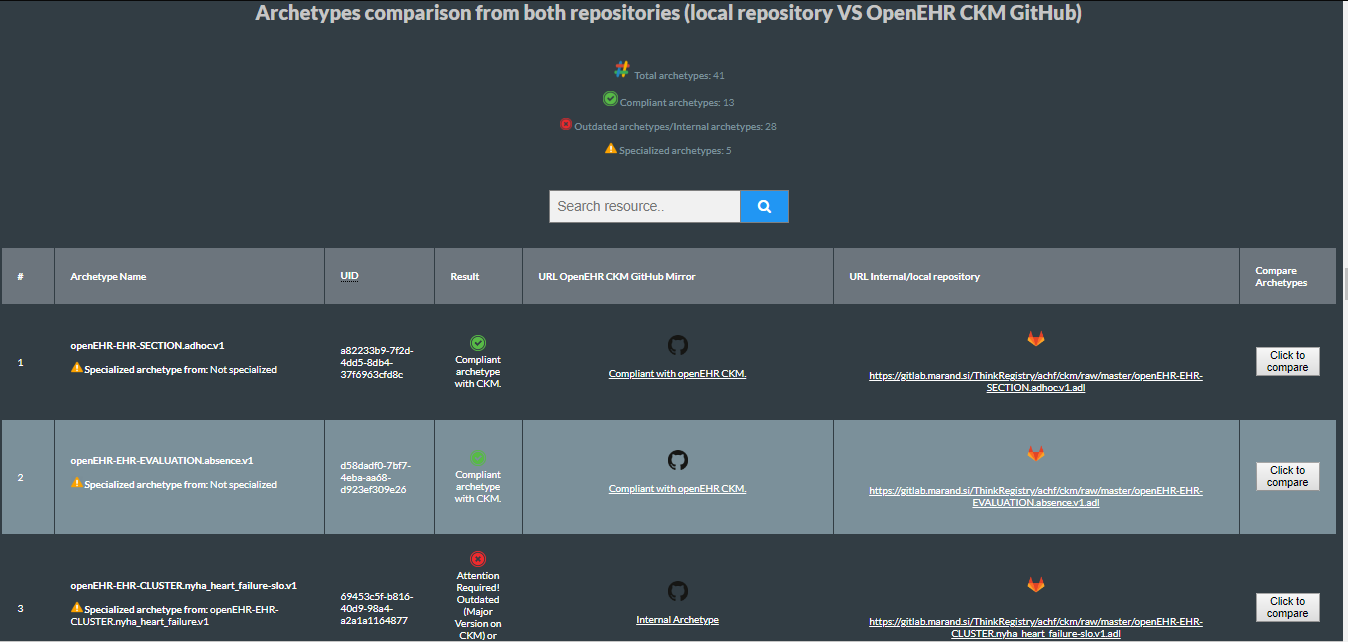
\includegraphics[width=1\textwidth]{img/arch_comparison.PNG}
	\caption{Module Comparison from local repository and compliance with the openEHR CKM mirror at Github}
	\label{fig:arch_comparison}
\end{figure}

On the top of each section, a resume from the analyzed process was made. Since the results obtained from the script were made by the archetype major version only (v.X), it was also made a comparison analysis with this information from the local repository provided for testing and the openEHR CKM mirror at GitHub. The result and comparison can be seen in tables \ref{tab:repos_comp_mv} and \ref{tab:comp_manual_script}, respectively.

\begin{table}[H]
	\centering
	\caption{Summary of archetype comparison analysis from the provided CKM repository with GitHub mirror of openEHR international CKM and the openEHR CKM by major version difference (June 2018) (n=41)}
	\label{tab:repos_comp_mv}
	\begin{tabular}{lll}
		\toprule[2pt]
		\multicolumn{3}{r}{\textbf{ Total (n=41) }} \\
		\cmidrule(r){2-3}
		\textbf{Archetype Status}   & \textbf{n} & \textbf{(\%)} \\
		\midrule[2pt]
		\textbf{Outdated } & 6 & (14,64) \\
		\midrule
		\textbf{Internal } & 16 & (39,02) \\
		\midrule
		\textbf{Not found } & 3 & (7,32) \\
        \midrule
		\textbf{Compliant } & 16 & (39,02) \\
		\bottomrule[2pt]
	\end{tabular}
\end{table}

When comparing the manual study made from the local repository to the openEHR CKM on GitHub to the developed script, the results are:

\begin{table}[H]
\centering
\caption{Comparison of the local repository analysis results retrieved by the manual analysis and the developed script. }
\label{tab:comp_manual_script}
\begin{tabular}{p{6cm} p{3cm} p{6.5cm}}
\toprule[2pt]
\textbf{ } & \textbf{Manual Analysis} & \textbf{Developed Script} \\ \midrule[2pt]
\textbf{Total archetypes}  & 41 & 41 \\ \midrule
\textbf{Compliant archetypes} & 16 & 14 \\ \midrule
\textbf{Not found archetypes} & 3 & N.A. \\ \midrule
\textbf{Outdated archetypes} & 6 & 6 \\ \midrule
\textbf{Internal archetypes} & 16 & 21 \\ \midrule
\textbf{Outdated or Internal archetypes} & N.A. & 27 (6 outdated, 21 internal, which are presented together in the script)
\\ \bottomrule[2pt]
\end{tabular}
\end{table}

The major differences from both analysis are presented in the number of compliant archetypes and internal archetypes. In the first case, it is due to the mirror errors from the openEHR CKM to the GitHub account during the committing process, where the archetypes \textit{openEHR-EHR-CLUSTER.healthcare\_provider\_parent} and \textit{openEHR-EHR-CLUSTER.address\_isa} have not been mirrored, and these causes a mislead to the script by recognizing them as internal archetypes. Other case that turns into misleading information, but in this case in the number of internal archetypes, are the archetypes whose archetype\_id have been renamed and cannot be found anymore on the openEHR CKM. These cases are:

\begin{itemize}[noitemsep]
\item \textit{openEHR-EHR-OBSERVATION.indirect\_oximetry} to \textit{openEHR-EHR-OBSERVATION.pulse\_oximetry};
\item \textit{openEHR-EHR-CLUSTER.timing\_repetition} to \textit{openEHR-EHR-CLUSTER.timing\_nondaily}.
\end{itemize}

In the next image, the second section is presented in detail, with some elements from the archetypes comparison list. Although the "red" alert for a outdated or internal archetype is appearing together, it can be understood that the archetype that is presented with and URL from GitHub in the next column, is a case of an outdated archetype. The next archetype on the list, is a case of an archetype that exists on the openEHR CKM, but it is not mirrored to the GitHub repository, which results on a "internal archetype" interpretation by the script.

\begin{figure}[H]
	\centering
    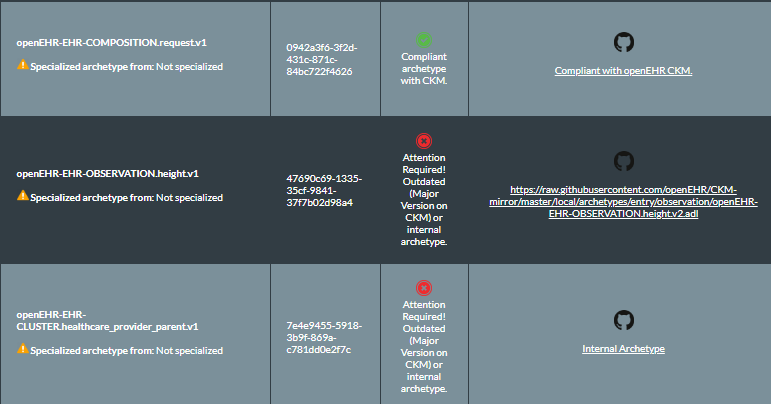
\includegraphics[width=1\textwidth]{img/arch_comparison_2.PNG}
	\caption{Detail from comparison module, with distinction from internal, outdated and compliant archetype}
	\label{fig:arch_comparison_2}
\end{figure}


The third section, was a internal request where the internship was made for improvement and future use case, which retrieve the list of templates and the set of archetypes included on those templates.

\begin{figure}[H]
	\centering
    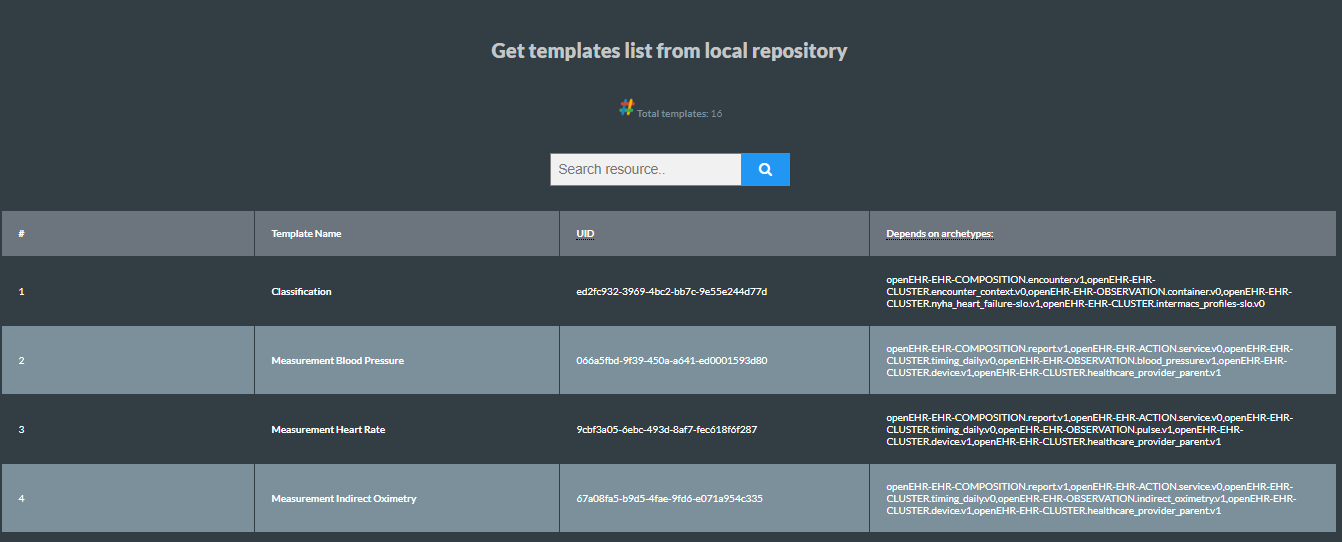
\includegraphics[width=1\textwidth]{img/get_temp_list.PNG}
	\caption{Module Get Templates list from local repository }
	\label{fig:get_temp_list}
\end{figure}

\subsection{Performance}

There was the opportunity to have the script been used and tested in three different projects by request. Two of them had an average of 50 archetypes and 10 templates and the other, an average of 670 archetypes and 190 templates. Since the script is dependent of ADL Designer REST API calls, for fetching the content from different repositories, they need to be connected previously to ADL Designer. Currently ADL Designer supports ADL versions 1.4 and 2 of archetypes and .OET format from templates, so if the resources are not well structured or have been edited manually on a text editor, without checking the consistence of data (which can compromise the structuring of these resources), or are saved on a different format, ADL Designer will not read them and automatically exclude this cases. The first two repositories had really "fresh" archetypes and templates, comparing with the third repository, that has resources dated from 2013 and with a lot of not recognized formats (.adls, .xml, .opt) by ADL designer, which provokes the exclusion of this cases when presenting the list of resources on the script. Also if an OET template is having in his sets of archetypes, an archetype that does not exists on the repository, it will also retrieve an error and not take this template on consideration. \\

The time taken for the script analysis in the third case was bigger, which took around 2,5 minutes to present all the page with the analysis and newer versions of archetypes available from GitHub, due to the higher number of resources, than in the first two cases, that only took 8 seconds to be completed. The speed of analysis can be quicker depending on the internet connection and the machine that is being used to run the script. This was tested on a machine with Intel i5 2nd generation processor with 6 GB of RAM with WI-FI access and a HDD drive, using Google Chrome version 68.0.3440.106 (64 bits).

\end{document}
